%%%%%%%%%%%%%%%%%%%%%%%%%%%%%%%%%%%%%%%%%
% Short Sectioned Assignment
% LaTeX Template
% Version 1.0 (5/5/12)
%
% This template has been downloaded from:
% http://www.LaTeXTemplates.com
%
% Original author:
% Frits Wenneker (http://www.howtotex.com)
%
% License:
% CC BY-NC-SA 3.0 (http://creativecommons.org/licenses/by-nc-sa/3.0/)
%
%%%%%%%%%%%%%%%%%%%%%%%%%%%%%%%%%%%%%%%%%

%----------------------------------------------------------------------------------------
%	PACKAGES AND OTHER DOCUMENT CONFIGURATIONS
%----------------------------------------------------------------------------------------

\documentclass[paper=a4, fontsize=11pt]{scrartcl} % A4 paper and 11pt font size

\usepackage[T1]{fontenc} % Use 8-bit encoding that has 256 glyphs
\usepackage{fourier} % Use the Adobe Utopia font for the document - comment this line to return to the LaTeX default
\usepackage[english]{babel} % English language/hyphenation
\usepackage{amsmath,amsfonts,amsthm} % Math packages

\usepackage[english]{babel}
\usepackage{graphicx}

\usepackage{lipsum} % Used for inserting dummy 'Lorem ipsum' text into the template

\usepackage{sectsty} % Allows customizing section commands
\allsectionsfont{\centering \normalfont} % Make all sections centered, the default font and small caps

\usepackage{fancyhdr} % Custom headers and footers
\pagestyle{fancyplain} % Makes all pages in the document conform to the custom headers and footers
\fancyhead{} % No page header - if you want one, create it in the same way as the footers below
\fancyfoot[L]{} % Empty left footer
\fancyfoot[C]{} % Empty center footer
\fancyfoot[R]{\thepage} % Page numbering for right footer
\renewcommand{\headrulewidth}{0pt} % Remove header underlines
\renewcommand{\footrulewidth}{0pt} % Remove footer underlines
\setlength{\headheight}{13.6pt} % Customize the height of the header

\numberwithin{equation}{section} % Number equations within sections (i.e. 1.1, 1.2, 2.1, 2.2 instead of 1, 2, 3, 4)
\numberwithin{figure}{section} % Number figures within sections (i.e. 1.1, 1.2, 2.1, 2.2 instead of 1, 2, 3, 4)
\numberwithin{table}{section} % Number tables within sections (i.e. 1.1, 1.2, 2.1, 2.2 instead of 1, 2, 3, 4)

\setlength\parindent{0pt} % Removes all indentation from paragraphs - comment this line for an assignment with lots of text

%----------------------------------------------------------------------------------------
%	TITLE SECTION
%----------------------------------------------------------------------------------------

\newcommand{\horrule}[1]{\rule{\linewidth}{#1}} % Create horizontal rule command with 1 argument of height

\title{	
\normalfont \normalsize 
\textsc{University of Southern California} \\ [25pt] % Your university, school and/or department name(s)
\horrule{0.5pt} \\[0.4cm] % Thin top horizontal rule
\huge CS402 Assignment 01 -- Performance \\ % The assignment title
\horrule{2pt} \\[0.5cm] % Thick bottom horizontal rule
}

\author{Michael Gerow} % Your name

\date{\normalsize\today} % Today's date or a custom date

\begin{document}

\maketitle % Print the title

%----------------------------------------------------------------------------------------
%	PROBLEM 1
%----------------------------------------------------------------------------------------

\section{Tests}
Getting the performance numbers of all the locking methods to line up with what one would "expect" them to be ended up being harder than I thought it would. I have two tests that I used to mark the performance of my locking implementations throughout development, but only one seems show fine being faster than rw being faster than coarse.

All of these tests make use of multiple processors to various degrees.  This is especially important because the only way to really gain additional performance from a machine with multiple processors is to write code that effectively uses more than one when locking and unlocking resources.

I also wrote a little python script to run tests multiple times and compute the mean and standard deviation of the runs.  These can be invoked with run\_unbalanced\_test.py and run\_gen\_test.py.

Also, all graphs that follow will have three vertical lines in them.  These represent the left standard deviation, the mean, and the right standard deviation.

\subsection{Unbalanced Test}
In order to get a result where fine is faster than rw is faster than coarse I really had to tune the test quite a bit. The way this test works is that it first initialzes the database with seven nodes in a perfectly balanced arrangement, leaving four leaves on the bottom of the tree.  I then had eight seperate threads make 50000 writes each that essentially made the tree incredibly imbalanced below those points. This alone was not enough to make sure that rw was faster than coarse, though, so I added eight extra threads that made essentially random reads throughout the database.  This had the effect of making rw fast enough to outpace coarse but now fast enough to beat fine.

This test can be invoked by running run\_unbalanced\_test.py with the only argument being the number of trials you would like to try.  This essentially pipes the file at test/unbalanced\_test into each of the server types.

\subsubsection{Data}
\begin{verbatim}
server_coarse	 mean: 8.3078	 standard deviation: 0.886419742099
server_rw	 mean: 7.2918	 standard deviation: 0.495389724956
server_fine	 mean: 5.2562	 standard deviation: 0.306972643865
\end{verbatim}

\subsubsection{Graphs}
\begin{figure}[h]
  \caption{A histogram of times taken by the coarse grained locking method for the unbalanced test} 
  \centering
  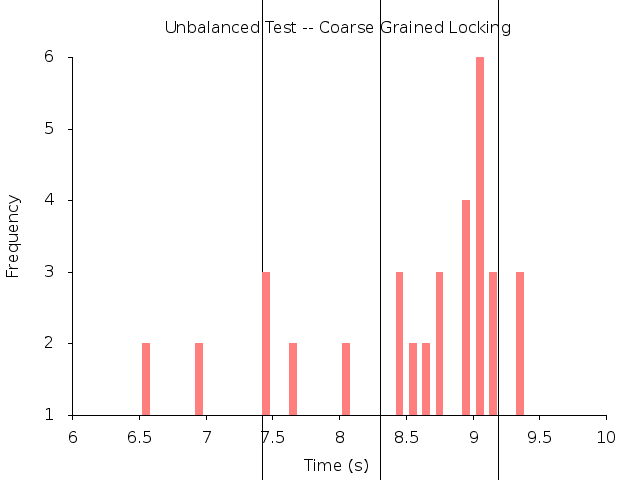
\includegraphics[width=\textwidth]{unbalanced_server_coarse_final.png}
  \label{fig:unbal_coarse}
\end{figure}

\begin{figure}[h]
  \caption{A histogram of times taken by the read write locking method for the unbalanced test} 
  \centering
  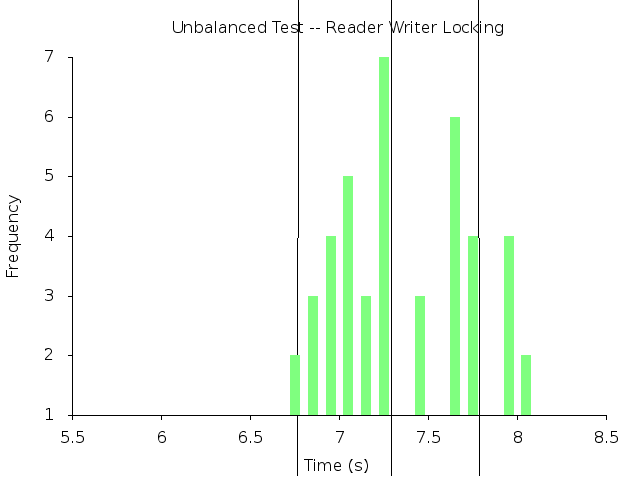
\includegraphics[width=\textwidth]{unbalanced_server_rw_final.png}
  \label{fig:unbal_rw}
\end{figure}

\begin{figure}[h]
  \caption{A histogram of times taken by the fine grained locking method for the unbalanced test} 
  \centering
  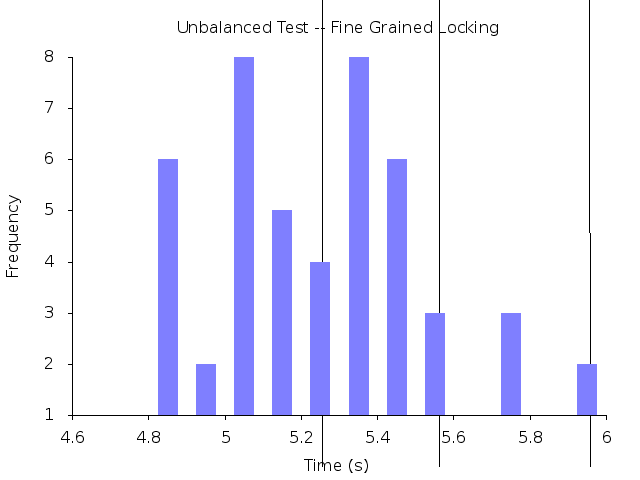
\includegraphics[width=\textwidth]{unbalanced_server_fine_final.png}
  \label{fig:unbal_fine}
\end{figure}
Please see \emph{figures} \ref{fig:unbal_coarse}, \ref{fig:unbal_rw}, and \ref{fig:unbal_fine}. 

\subsubsection{Analysis}
We can clearly see that the performance ranks in expected order, that is that fine grained locking beats read write locking which beats coarse grained locking.

The reason fine grained locking seems to work so well in this scenario is because each of the eight writing threads essentially stick to their own part of the tree, making it easy for multiple threads to be writing to the tree at the same time.  Read write, on the other hand, can only have one thread writing to the tree at once time.  It is able to beat the coarse grained lock, though, because there is also a collection of reads in the test that the rw method is able to execute mostly in parallel while the coarse grained lock must serialize these accesses.

I would like to note, though, that this test took a fair amount of tweaking in order to get these results. For most random inputs it seems that the fine grained locking loses out to read write locking, as we will see in the next test. 

\subsection{Gen Test}
This next test I called the "gen" test, mainly because it is generated randomly from the files in test/readergen.py and test/writergen.py.  These scripts generate 50000 random reads between 0 and 16536 and 16536 random writes that go from 0 to 16536 (essentially hitting all values in the range).  This test is read heavy, which I thought might somewhat closely model a database used in an application like a web server, so I thought it would be an interesting test case to look at.

As with the unbalanced test this test can be invoked by running run\_gen\_test.py with the only argument being the desired number of trials per server type. It essentially pipes the file at test/gen\_test into each of the server types.

\subsubsection{Data}
\begin{verbatim}
server_coarse	 mean: 5.759	 standard deviation: 0.582357103433
server_rw	 mean: 2.15	 standard deviation: 0.311028576678
server_fine	 mean: 3.0696	 standard deviation: 0.116495773769
\end{verbatim}

\subsubsection{Graphs}
\begin{figure}[h]
  \caption{A histogram of times taken by the coarse grained locking method for the gen test} 
  \centering
  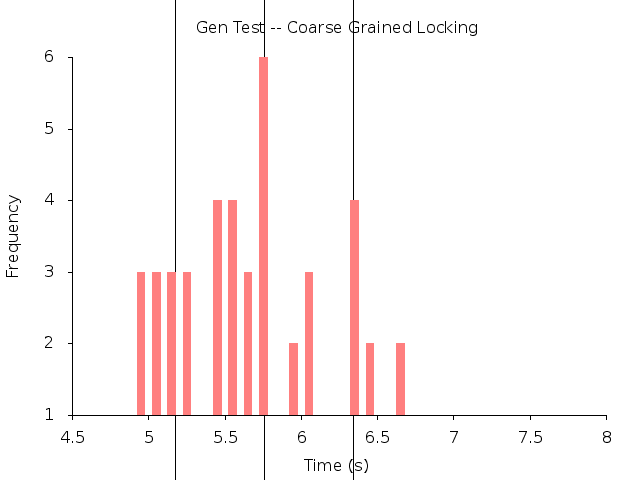
\includegraphics[width=\textwidth]{gen_server_coarse_final.png}
  \label{fig:gen_coarse}
\end{figure}

\begin{figure}[h]
  \caption{A histogram of times taken by the read write locking method for the gen test} 
  \centering
  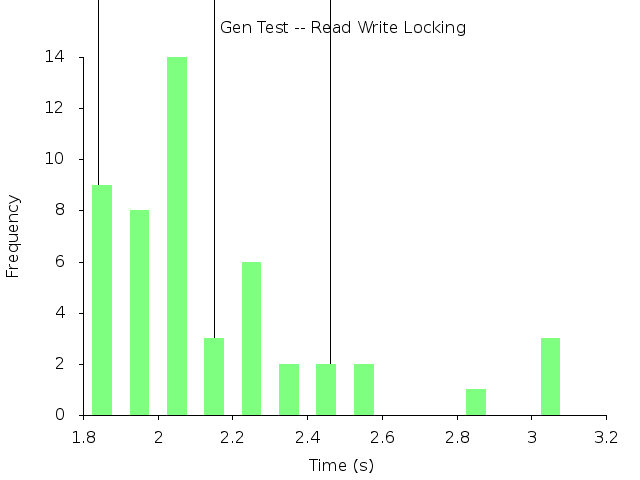
\includegraphics[width=\textwidth]{gen_server_rw_final.png}
  \label{fig:gen_rw}
\end{figure}

\begin{figure}[h]
  \caption{A histogram of times taken by the fine grained locking method for the gen test} 
  \centering
  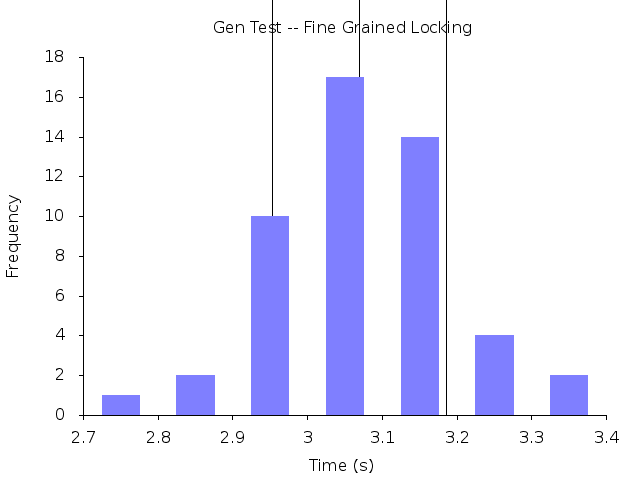
\includegraphics[width=\textwidth]{gen_server_fine_final.png}
  \label{fig:gen_fine}
\end{figure}
Please see \emph{figures} \ref{fig:gen_coarse}, \ref{fig:gen_rw}, and \ref{fig:gen_fine}. 

\subsubsection{Analysis}
Somewhat unexpectedly, the fine grained locking seems to be losing out to the read write locking by a significant amount.  One would expect a finer grain of lock would almost always result in an increase in performance, but this test seems to turn that on its head.

I have not done an extremely thorough exploration about why this might happen, but I can take a guess. It is likely that the fine grained lock happens to block a lot in the middle of reading the tree in order to wait on a lock to be freed.  The overhead associated with constant blocking and unblocking may ultimately be too much to really beat the less fine grained read write locking.

All that time the read write locking method is sending entire queries through the table without there even being a possibility of blocking midway through the table, eliminating the overhead that can bring.

\end{document}
